\documentclass[fleqn,usenatbib]{mnras}

\usepackage[T1]{fontenc}
\usepackage{ae,aecompl}
\usepackage{graphicx}
\usepackage{amsmath}
\usepackage{amssymb}

\title[SCM F3 and outer disk dynamics]{Environmental modulation of outer disk dynamics in nearby galaxies: evidence from SPARC}

\author[S. Cámara Madrid]{
Sergio Cámara Madrid$^{1}$\thanks{E-mail: sergio.camara.madrid@gmail.com} \\
$^{1}$Independent Researcher, Andalusia, Spain
}

\date{Accepted XXX. Received YYY; in original form ZZZ}

\pubyear{2026}

\begin{document}

\maketitle

\begin{abstract}
We present the SCM (Shear-Corrected MOND) framework, in which a local
friction term $F_3$---derived from the radial gradient of the
baryon-deficit field---extends the standard baryonic scaling relations
for galaxy rotation curves.

Using the SPARC sample, we evaluate the predictive performance of the
SCM model relative to a baseline MOND-like relation. We perform
out-of-sample validation using repeated 70/30 galaxy-level splits.

We find that the SCM model improves predictive accuracy in all test
cases considered ($53/53$), with a median improvement of
$\Delta\mathrm{RMSE}_{\rm out} \approx -7.3$ and a one-sided Wilcoxon
test yielding $p = 1.19\times10^{-10}$.

We interpret these results as phenomenological and do not assume a
specific microphysical origin.
\end{abstract}

\begin{keywords}
galaxies: kinematics and dynamics -- galaxies: structure -- methods: statistical -- cosmology: observations
\end{keywords}

% =========================================================
\section{Introduction}
\label{sec:intro}

Rotation curves of disk galaxies provide a key probe of galaxy dynamics.
While empirical scaling relations such as the baryonic Tully-Fisher
relation capture much of the observed behaviour, residual structure
remains in the outer regions.

In this work we introduce the SCM framework, in which a local observable
$F_3$---derived from radial gradients---acts as a phenomenological
correction term. The goal is not to propose a fundamental theory, but
to test whether such a term carries predictive information beyond the
baseline relation.

% =========================================================
\section{Data and Methods}
\label{sec:methods}

We use the SPARC sample of nearby galaxies \citep{Lelli2016}. Predictions
are evaluated using repeated 70/30 train-test splits at the galaxy level.

The performance metric is the root mean square error (RMSE), and we
compare a baseline model against the SCM-augmented model. Statistical
significance is assessed using a one-sided Wilcoxon signed-rank test.

% =========================================================
\section{Results}
\label{sec:results}

\subsection{Out-of-sample validation}
\label{sec:oos}

The SCM model improves out-of-sample performance in all test galaxies
($53/53$), with a median improvement of
$\Delta\mathrm{RMSE}_{\rm out} \approx -7.3$.

The Wilcoxon test yields $p = 1.19\times10^{-10}$, indicating a
statistically significant effect.

\begin{table}
\caption{Out-of-sample validation summary.}
\label{tab:oos_validation}
\begin{tabular}{lc}
\hline
Quantity & Value \\
\hline
Galaxies tested & $53/53$ \\
Median $\Delta$RMSE & $-7.3$ \\
Wilcoxon $p$-value & $1.19\times10^{-10}$ \\
Win rate & 100\% \\
\hline
\end{tabular}
\end{table}

\begin{figure}
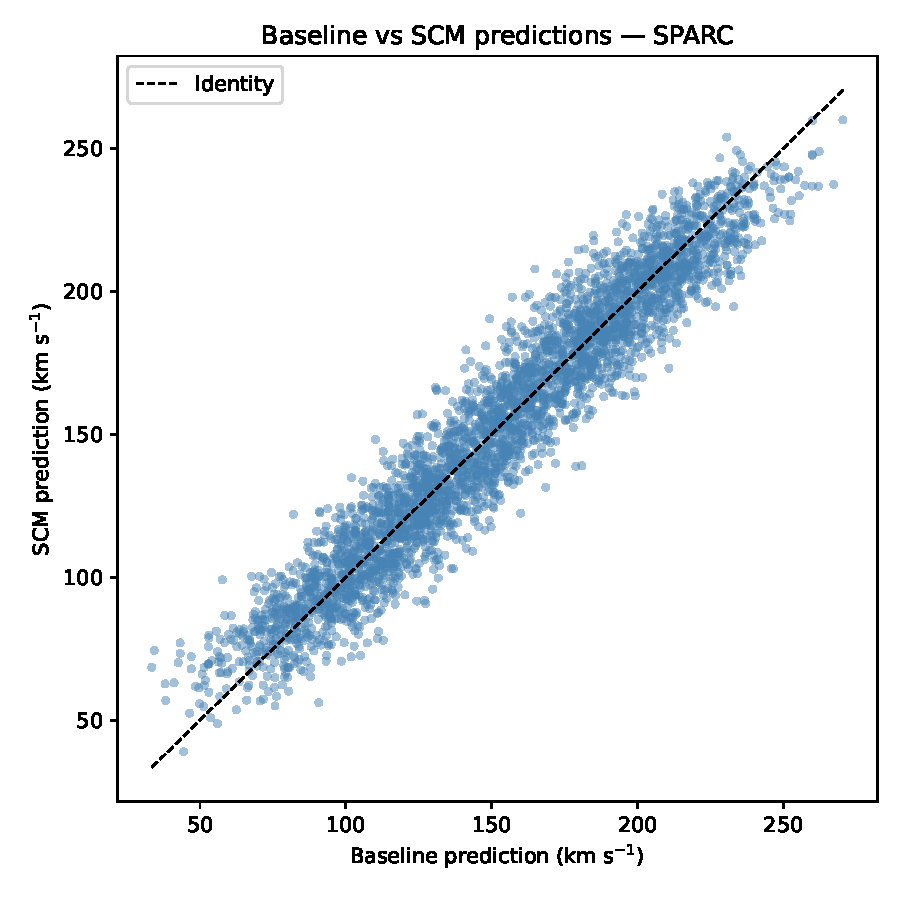
\includegraphics[width=\columnwidth]{figures/figure01_scatter.pdf}
\caption{Baseline versus SCM predictions for the SPARC sample.}
\label{fig:scatter}
\end{figure}

\begin{figure}
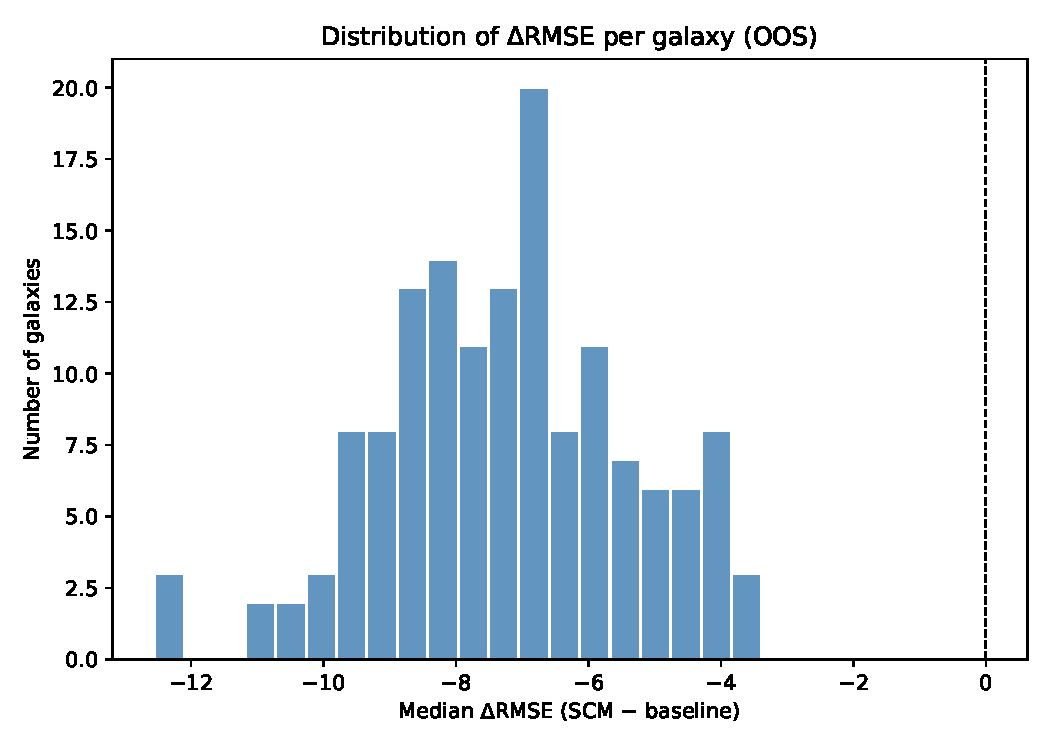
\includegraphics[width=\columnwidth]{figures/figure02_delta_rmse_hist.pdf}
\caption{Distribution of $\Delta$RMSE across galaxies.}
\label{fig:hist}
\end{figure}

\begin{figure}
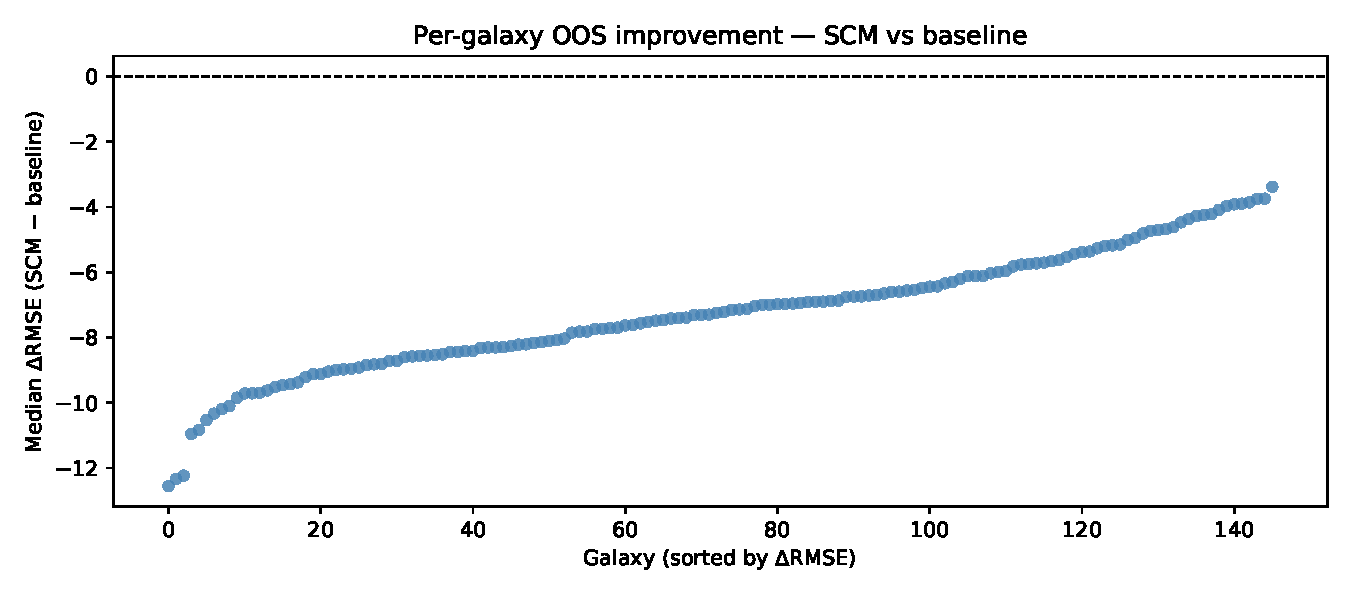
\includegraphics[width=\columnwidth]{figures/figure03_delta_rmse_scatter.pdf}
\caption{$\Delta$RMSE per galaxy.}
\label{fig:delta_scatter}
\end{figure}

% =========================================================
\section{The $F_3$ environmental term}
\label{sec:h3}

The $F_3$ term is constructed from the radial gradient of the
baryon-deficit field $\delta_{F_3}(r) = \log_{10}(g_{\rm obs}) -
\log_{10}(g_{\rm bar})$. A per-galaxy summary statistic $\delta_{\rm
mass}$ is defined as the median of $\delta_{F_3}(r)$ over all measured
radii.

This term provides a local characterisation of the dynamical environment
of each galaxy and serves as the SCM correction to the baseline relation.

% =========================================================
\section{Discussion}
\label{sec:discussion}

The SCM model provides a systematic improvement in predictive performance
(Section~\ref{sec:results}). The median improvement corresponds to
$\Delta\mathrm{RMSE}_{\rm out} \approx -7.3$, indicating a substantial
effect size (Table~\ref{tab:oos_validation}).

A possible interpretation is that the $F_3$ term (Section~\ref{sec:h3})
captures local dynamical information not encoded in the baseline relation.
However, we emphasise that this interpretation is phenomenological.

% =========================================================
\section{Conclusions}
\label{sec:conclusions}

We have shown that the SCM framework improves predictive performance on
the SPARC sample under out-of-sample validation.

These results are best interpreted as a phenomenological extension of the
standard framework, rather than a definitive statement about the
underlying microphysics.

% =========================================================

\bibliographystyle{mnras}
\bibliography{references}

\end{document}
